\documentclass[12pt, a4paper]{report}
\usepackage[utf8]{inputenc}
\usepackage[T1]{fontenc}
\usepackage[utf8]{inputenc}
\usepackage{geometry}
\usepackage{listings}
\usepackage{xcolor}
\usepackage[]{graphicx}
\usepackage[export]{adjustbox}
\usepackage{subcaption}
\makeatletter
\setlength{\@fptop}{0pt}
\makeatother

\definecolor{codegreen}{rgb}{0.26, 0.61, 0}
\definecolor{codegray}{rgb}{0.5,0.5,5}
\definecolor{codepurple}{rgb}{58,0,0.82}
\definecolor{backcolour}{rgb}{0.80, 0.81, 0.93}

\lstdefinestyle{mystyle}{
    backgroundcolor=\color{backcolour},   
    commentstyle=\color{codegreen},
    keywordstyle=\color{magenta},
    numberstyle=\tiny\color{codegray},
    stringstyle=\color{codepurple},
    basicstyle=\ttfamily\footnotesize,
    breakatwhitespace=false,         
    breaklines=true,                 
    captionpos=b,                    
    keepspaces=true,                 
    numbers=left,                    
    numbersep=5pt,                  
    showspaces=false,                
    showstringspaces=false,
    showtabs=false,                  
    tabsize=2
}

\lstset{style=mystyle}


\title{\textbf{EE2703: Applied Programming Lab\\Assignment 6B\\Laplace Tranform
}}


\author{Devaganthan S S\\ EE19B018}
\date{\today}
\begin{document}

\maketitle


\section{Abstract}
This assignment aims to analyze “Linear Time-Invariant Systems” with numerical tools in python.

\section{Introduction}
LTI systems are an important part of Electrical Engineering. Python has a Signals toolbox, which enables engineers to analyze LTI systems efficiently. In this assignment, we take different problems and use the functions such as \textbf{sp.lti , sp.impulse , sp.lsim } to solve them.
\section{Results and Implementation}
\subsection{Spring Mass System:}
We apply a time varying (Sinusoidal and Decaying) force to a spring mass system. We need to find position of the mass (x) as function of time. We take the Laplace form of the given differential equation, to find the Laplace Transform of x(t). Using \textbf{sp.lti()}, we find x(t). The below code accomplishes the above tasks, and plots x(t) vs time graph
\noindent
\lstinputlisting[language = python]{code1.py}
\begin{figure}[h!]
    \centering
    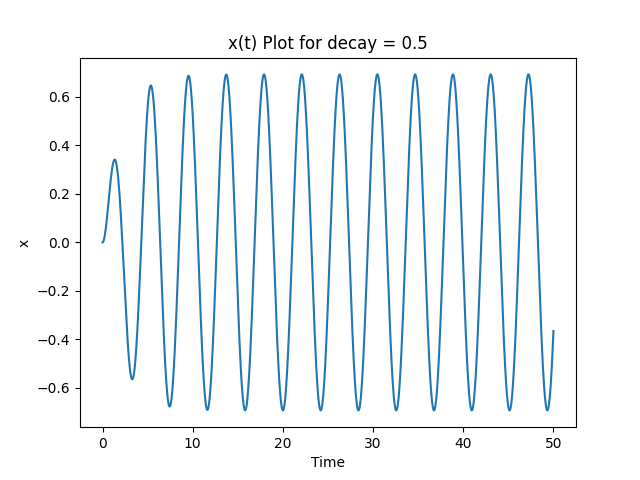
\includegraphics[scale=0.75]{fig1.png} 
    \caption{Position of mass as function of time}
    \label{fig:my_label}
\end{figure}
\vspace{100mm}
\subsection{With a Smaller Decay}
We repeat the same as before with a different decay rate. The below code accomplishes the above tasks, and plots the new x(t) vs time graph.



\lstinputlisting[language = python]{code2.py}
\begin{figure}[h!]
    \centering
    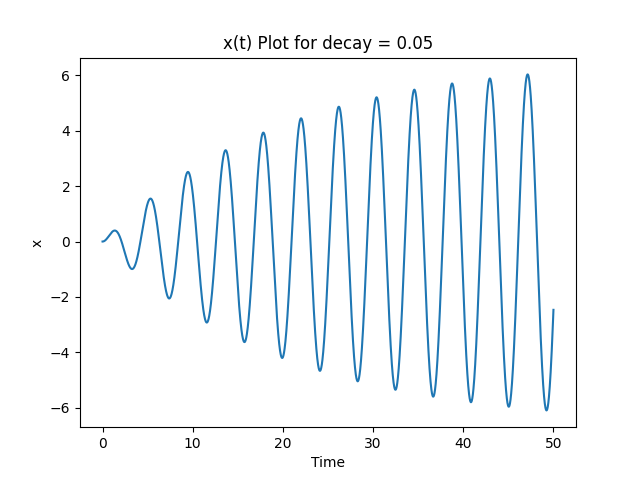
\includegraphics[scale=0.75]{fig2.png} 
    \caption{Position of mass as function of time}
    \label{fig:my_label}
\end{figure}
\vspace{100mm}
\subsection{Varying the Frequency of the Sinusoid:}
We consider the problem to be an LTI system with f(t) as the Input and x(t) as the output.We vary the Frequency of the Sinusoid from 1.4 to 1.6 in steps of 0.05, to see how x(t) varies. We use the function \textbf{sp.lsim} to compute the output. The amplitude of the output is maximum at its Natural Frequency of 1.5. The below code accomplishes the above tasks and plots the frequency variation of the Ouptut.
\noindent
\lstinputlisting[language = python]{code3.py}
\begin{figure}[h!]
    \centering
    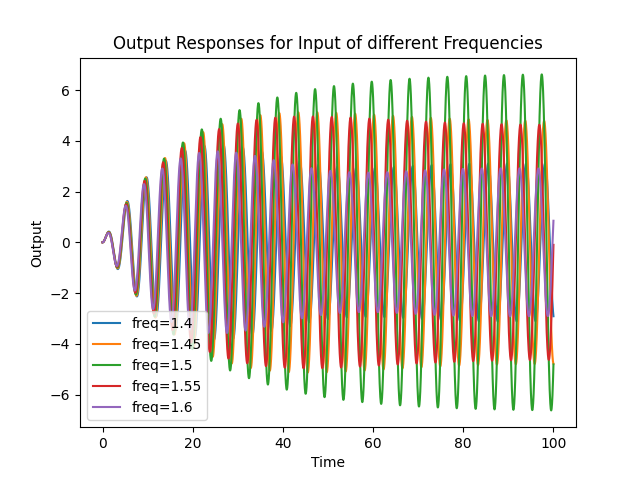
\includegraphics[scale=0.75]{fig3.png} 
    \caption{}
    \label{fig:my_label}
\end{figure}
\subsection{Coupled Spring Problem}
From the given Differential Equations and Initial Conditions, we find,
\begin{equation}
X(s) = \frac{s^2+2}{s^3+3s}
\end{equation}
\begin{equation}
Y(s) = \frac{2}{s^3+3s}
\end{equation}
We find x(t) and y(t) using the function \textbf{sp.lsim()}. The below code accomplishes the above tasks and plots x(t) and y(t) as function of time.
\noindent
\lstinputlisting[language = python]{code4.py}
\begin{figure}[h!]
    \centering
    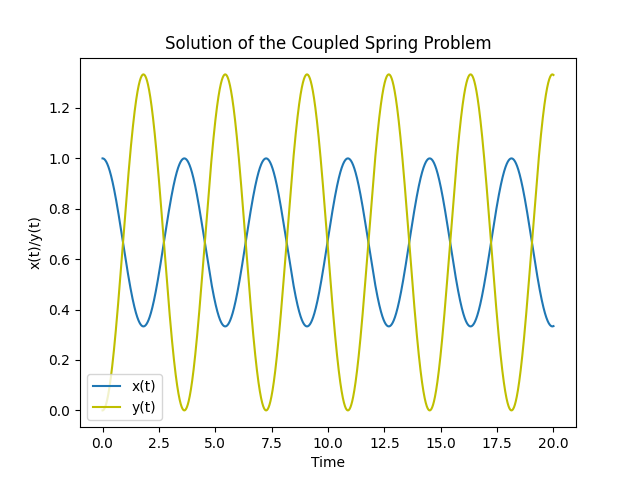
\includegraphics[scale=0.75]{fig4.png} 
    \caption{}
    \label{fig:my_label}
\end{figure}
\subsection{Two Port Network:}
The transfer Function of the two port network is,
\begin{equation}
H(s) = \frac{1}{LCs^2 + RCs + 1}
\end{equation}
We use the function \textbf{bode()} and \textbf{sp.lti()} to compute values of the magnitude and phase for different frequencies. The below code accomplishes the above tasks and plots the Bode plot for the Transfer Function found.
\vspace{100mm}
\noindent
\lstinputlisting[language = python]{code5.py}
\begin{figure}[h!]
    \centering
    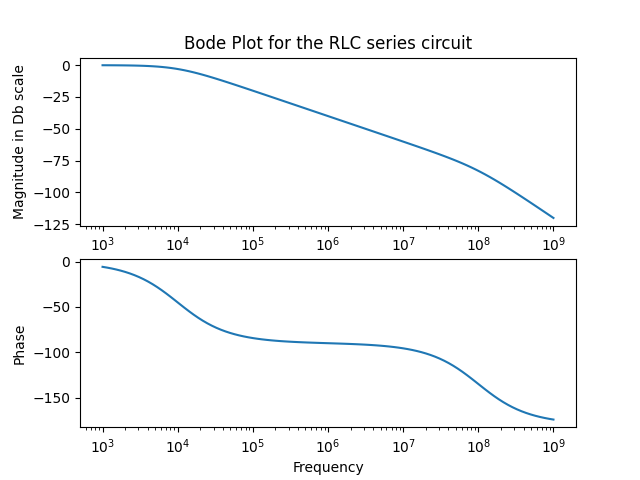
\includegraphics[scale=0.75]{fig5.png} 
    \caption{}
    \label{fig:my_label}
\end{figure}
\subsection{Finding the Output for the given input for the Two Port System:}
The Output to the given Input can be  found using the \textbf{sp.lsim()} function. We plot the output over both small and large time scale to better understand the variations. The below code accomplishes the above tasks.
\vspace{2mm}
\noindent
\lstinputlisting[language = python]{code6.py}
\begin{figure}[h!]
    \centering
    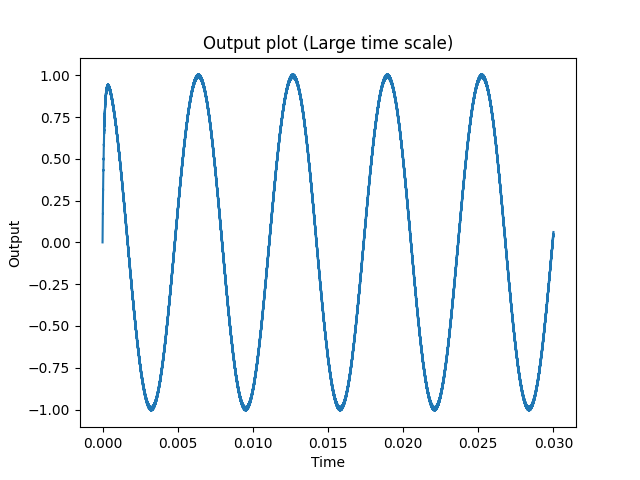
\includegraphics[scale=0.75]{fig6.png} 
    \caption{}
    \label{fig:my_label}
\end{figure}
\vspace{10mm}
\lstinputlisting[language = python]{code7.py}
\begin{figure}[h!]
    \centering
    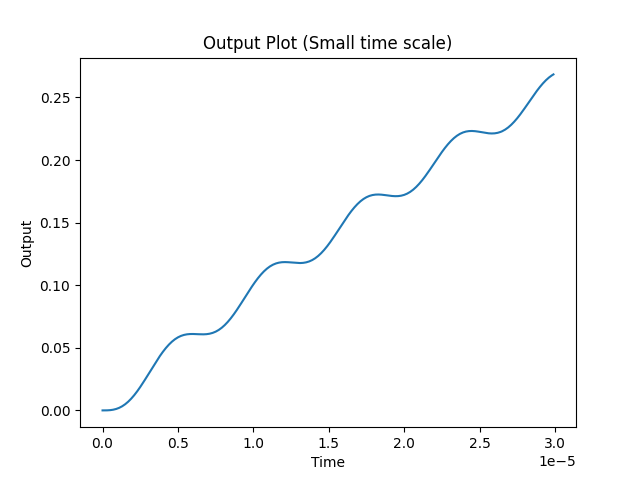
\includegraphics[scale=0.75]{fig7.png} 
    \caption{}
    \label{fig:my_label}
\end{figure}
\section{Conclusion}
We have Analyzed "Linear Time-Invariant systems" with Numerical tools in Python. We learnt how to use functions like sp.lti(), sp.impulse(), sp.lsim().


\end{document}

